\subsubsection{\theoryC{High mass dilepton searches at HE-LHC ($ee, \mu\mu, \tau\tau$)}}
\label{subsubsec:hr_lep}
\contributors{C. Helsens, D. Jamin, M. Selvaggi}\rt{There are comments to address.}

\newcommand*{\sqrtshelhc}{\ensuremath{\sqrt{s}=\text{27 TeV}}}


%{\bf Authors: C. Helsens$^1$, D. Jamin$^2$, M. Selvaggi$^3$}\\
%\newline
%$^1$CERN EP-Departement, CH-1211 Geneva 23, Switzerland email: {\tt B.C. clement.helsens@cern.ch}\\
%$^2$Academia Sinica, Institute of  Physics, Taipei, Taiwan\\


%\newcommand*{\Zp}{\ensuremath{Z^{\prime}}}
%\newcommand*{\ZpSSM}{\ensuremath{Z^{\prime}_{\mathrm{SSM}}}}
%\newcommand*{\Z}{\ensuremath{Z}}
%\newcommand*{\Zptata}{\ensuremath{Z^{\prime}\rightarrow \tau\tau}}
%\newcommand*{\Zpee}{\ensuremath{Z^{\prime}\rightarrow e e}}
%\newcommand*{\Zpmumu}{\ensuremath{Z^{\prime}\rightarrow \mu\mu}}
%\newcommand*{\Zpll}{\ensuremath{Z^{\prime}\rightarrow \ell\ell}}
%\newcommand*{\Zptt}{\ensuremath{Z^{\prime}\rightarrow \ttbar}}
%\newcommand*{\ptZp}{\ensuremath{p_{\text{T}}^{\ensuremath{Z^{\prime}}}}}
%\newcommand*{\intlumihelhc}{\ensuremath{\mathcal{L}=15\text{ ab}^{-1}}}


%%%%%%%%%%%%%%%%%%%%%%%%%%%%%%%%%%%%%%%%%%%%%%%%%%%%%%%%%%%%%%%%%%%%%%%%%%%%%%%%%%%%%%%%%%%%
%\subsubsection{Introduction}
%\paragraph*{Introduction}
Models with extended gauge groups often feature additional U(1) symmetries with corresponding heavy spin-1 bosons. These bosons, generally referred to as $\Zp$, would manifest themselves as a narrow resonance in the dilepton invariant mass spectrum. Among these models are those inspired by Grand Unified Theories, motivated by gauge unification, or a restoration of the left-right symmetry violated by the weak interaction. Examples include the $\Zp$ bosons of the $E_{6}$ motivated theories~\cite{London:1986jz,Joglekar:2016yap,Langacker:2008yv} and Minimal models~\cite{Salvioni:2009mt}. The Sequential Standard Model (SSM)~\cite{Langacker:2008yv} posits a $\ZpSSM$ boson with couplings to fermions that are identical to those of the Standard Model $\Z$ boson.

The decay products of heavy resonances are in the multi-TeV regime and the capability to reconstruct their momentum imposes stringent requirement on the detector design. In particular, reconstructing the track curvature of multi-TeV muons requires excellent position resolution and a large lever arm. In this section, the expected sensitivity is presented for a \Zpll\ (where $\ell=\mathrm{e},\mu$) and \Zptata\ separately.

%%%%%%%%%%%%%%%%%%%%%%%%%%%%%%%%%%%%%%%%%%%%%%%%%%%%%%%%%%%%%%%%%%%%%%%%%%%%%%%%%%%%%%%%%%%%
%\subsubsection{Monte Carlo Samples}
%\paragraph*{Monte Carlo Samples}
Monte Carlo simulated event samples were used to simulate the response of the future detector to signal and backgrounds. The muon momentum resolution is assumed to be $\sigma(p)/p \approx 10\%$ at $\pt~=~5$~TeV for central muons. Signals are generated with \pythia~8.230~\cite{Sjostrand:2014zea} using the leading order cross-section from the generator.
All lepton flavour decays of the $\ZpSSM$ are generated assuming universality of the couplings.
The Drell-Yan background has been generated using \MGvATNLO 2.5.2~\cite{Alwall:2014hca} at leading order only. A conservative overall k-factor of 2 has been applied to all the background processes to account for possible higher order QCD corrections.\rt{In every contribution you put a $k$-factor of 2 on the background. This seems an irrelevant arbitrary assumption.}

%%%%%%%%%%%%%%%%%%%%%%%%%%%%%%%%%%%%%%%%%%%%%%%%%%%%%%%%%%%%%%%%%%%%%%%%%%%%%%%%%%%%%%%%%%%%
%\subsubsection{Event Selection}
%\paragraph*{Event Selection}
For the $\ell\ell$ final-states events are required to contain two isolated leptons with $\pt > 500$~GeV and $|\eta|<4$. For the $\tau\tau$ final state we focus solely on the fully hadronic decay mode which is expected to drive the sensitivity. The $\tau\tau$ event selection requires the presence two reconstrcuted jets with $\pt > 500$~GeV and $|\eta|<2.5$ identified as hadronic $\tau$'s. To ensure orthogonality between the $\ell$ and $\tau$ final states, jets overlapping with isolated leptons are vetoed. Additionnal mass dependent selection criteria on the azimutal angle between the two reconstructed $\tau$'s are applied to further improve the QCD background rejection (see \tabb{tab:leptonicresonances:selectiontautau}).

The left and central panels of \fig{fig:leptonicresonances:masses} show the invariant mass distribution for a 6~TeV $\ZpSSM$ in the $ee$ and $\mu\mu$ channels. The mass resolution is better for the $ee$ channel, as expected. The right panel of \fig{fig:leptonicresonances:masses} shows the transverse mass~\footnote{The transverse mass is defined as $m_{T}  =  \sqrt{2\ptZp*\met*(1-\cos\Delta\phi(\Zp,\met))}$.}
of a 6~TeV signal for the $\tau\tau$ channel. Because of the presence of neutrinos in $\tau$ decays, the true resonance mass cannot be reconstructed. Several arbitrary  choices are possible to approximate the $Z'$ mass. The transverse mass provided the best sensitivity and was therefore used to set limits and determine the discovery reach in $\tau\tau$ decay mode.

\begin{table}[htbp]
   \centering
\begin{tabular}{l|l|c|r}
   $\Zp$ mass [TeV] &  $\Delta \phi(\tau_1, \tau_2)$&  $\Delta R(\tau_1, \tau_2)$ & $\met$\\
  \hline
   $2$ & > 2.4 & > 2.4 and < 3.9 & > 80 GeV\\
   $4$ & > 2.4 & > 2.7 and < 4.4 & > 80 GeV\\
   $6$ & > 2.4 & > 2.9 and < 4.4 & > 80 GeV\\
   $8$ & > 2.6 & > 2.9 and < 4.6 & > 80 GeV\\
  $10$ & > 2.8 & > 2.9 and < 4.1 & > 60 GeV\\
  $12$ & > 2.8 & > 3.0 and < 3.6 & > 60 GeV\\
  $14$ & > 3.0 & > 3.0 and < 3.3 & > 60 GeV\\
  \end{tabular}
  \caption{List of mass dependent cuts optimised to maximise the sensitivity for the \Zptata\ search.}
  \label{tab:leptonicresonances:selectiontautau}
\end{table}


\begin{figure}[htbp]
  \centering
  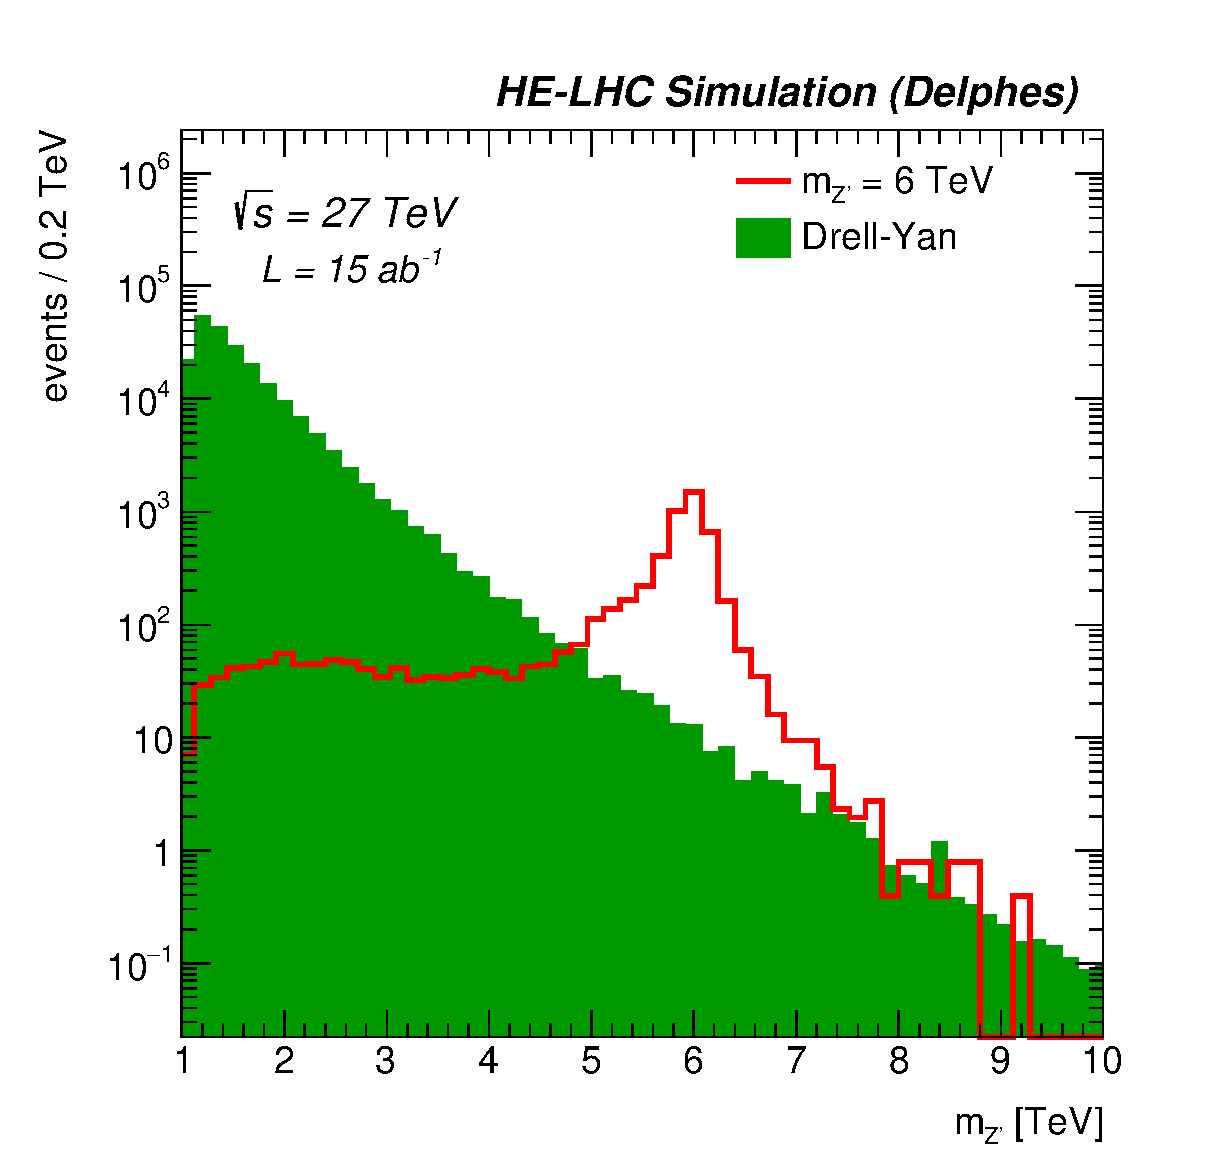
\includegraphics[width=0.32\columnwidth]{\main/section7OtherSignatures/img/Zpee_mzp_sel0_nostack_log.eps}
  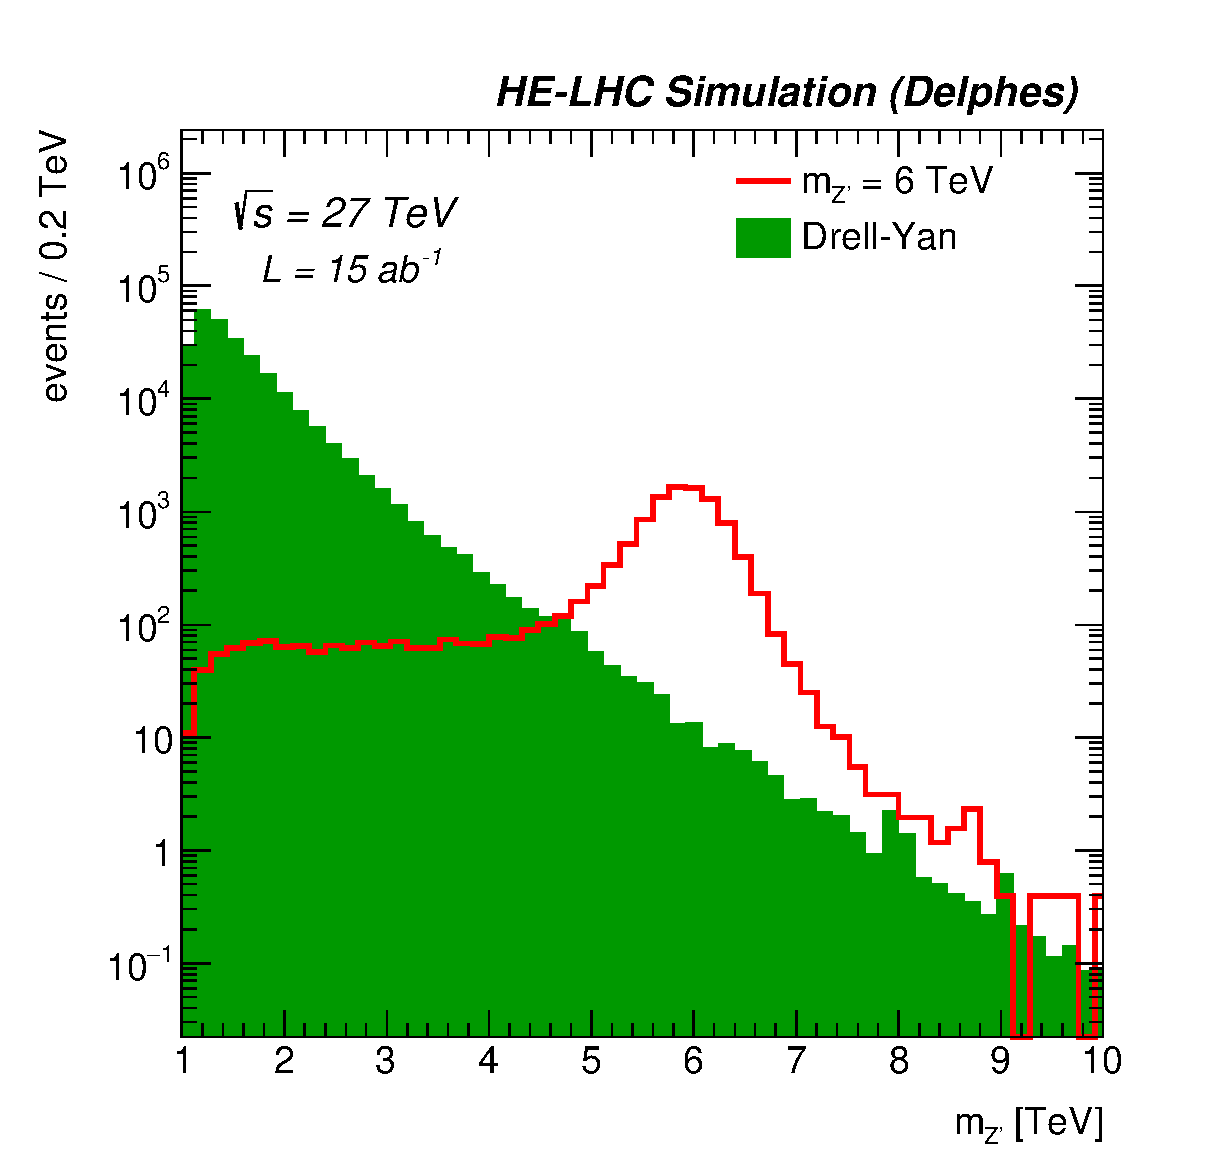
\includegraphics[width=0.32\columnwidth]{\main/section7OtherSignatures/img/Zpmumu_mzp_sel0_nostack_log.eps}
  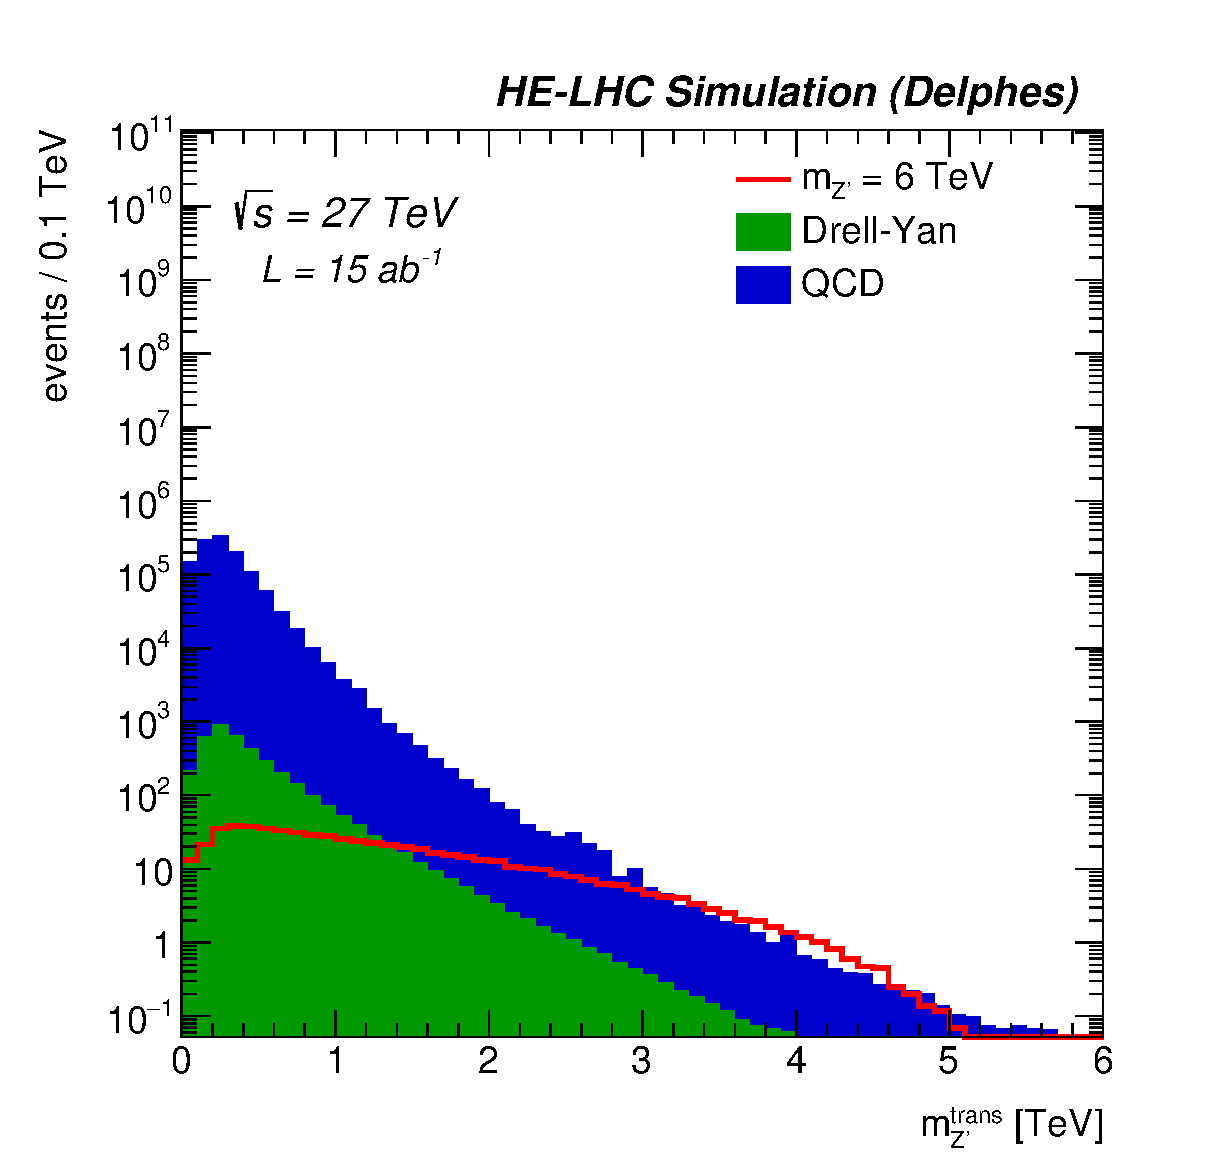
\includegraphics[width=0.32\columnwidth]{\main/section7OtherSignatures/img/Zptautau_mt_sel0_nostack_log.eps}
  \caption{Left, center: Invariant mass for a 6~TeV signal after full event selection for ee channel (left) and $\mu\mu$ channel (center). Right: Transverse mass for a 6~TeV signal after full event selection for the $\tau\tau$ channel. }
  \label{fig:leptonicresonances:masses}
\end{figure}
%\MS{need editing / style}

%%%%%%%%%%%%%%%%%%%%%%%%%%%%%%%%%%%%%%%%%%%%%%%%%%%%%%%%%%%%%%%%%%%%%%%%%%%%%%%%%%%%%%%%%%%%
%\subsubsection{Results and discussion}
%\paragraph*{Results and discussion}
Hypothesis testing is performed using a modified frequentist method based on a profile likelihood that takes into account the systematic uncertainties as nuisance parameters that are fitted to the expected background predicted from Monte Carlo. For the $ee$ and $\mu\mu$ analyses, the dilepton invariant mass is used as the discriminant, while for the $\tau\tau$ channel the transverse mass is used. A 50\% uncertainty on the background normalisation is assumed.

The 95\% C.L. exclusion limit obtained using \intlumihelhc\ of data for the combination of the ee and $\mu\mu$ channels is shown in \fig{fig:leptonicresonances:resultsll} (left) for a list of 6 different $Z'$ models. A detailed discussion on model discrimination at HE-LHC following the observation of an excess at the HL-LHC can be found in Section~\ref{sec:modeldiscr}. We simply note here that it is possible to exlude a $Z'$ with $m_{Z'}\lesssim 10-12$~TeV (depending on the model) at \sqrtshelhc\ with \intlumihelhc. Figure~\ref{fig:leptonicresonances:resultsll} (right) shows the integrated luminosity required to reach a $5\sigma$ discovery for a $\ZpSSM$ decaying leptonically as a function of the mass of the heavy resonance. Despite a worse di-lepton invariant mass resolution for the $\mu\mu$ final state, the \Zpee\ and \Zpmumu\ channel display very similar performances, due to the low background rates and a higher muon reconstruction efficiency. With the full dataset \intlumihelhc, a $\ZpSSM$ up to $m_{Z'}\approx 13$~TeV can be discovered.  Figure~\ref{fig:leptonicresonances:resultstautau} shows the exclusion limits for 15 ab$^{-1}$ of data (left) and the required integrated luminosity
versus mass to reach a $5\sigma$ discovery (right) for the $\tau\tau$ resonances. We find that a $\ZpSSM$ with $m_{Z'}\approx 6.5$~TeV can be discovered or excluded. As expected, the \Zptata\ final-state yields to a worse discovery potential compared to the $\ell\ell$ final states because of the presence of a much larger background contribution as well as the absence of narrow mass peak.

  \begin{figure}[htbp]
  \centering
  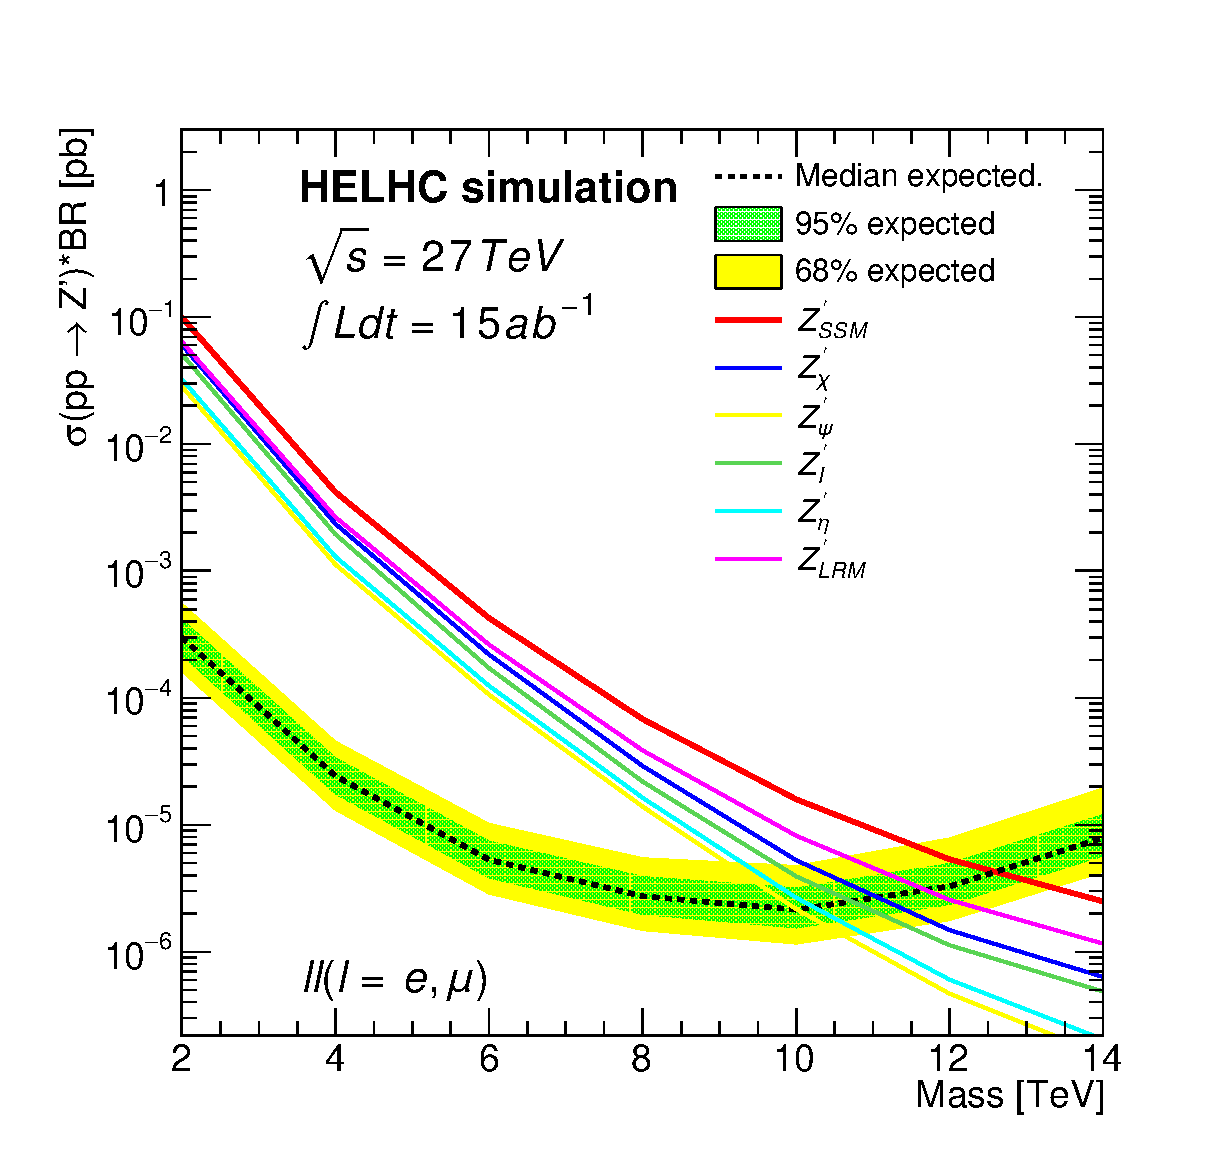
\includegraphics[width=0.45\columnwidth]{\main/section7OtherSignatures/img/lim_Zprime_ll_helhc_v01_allxs.eps}
  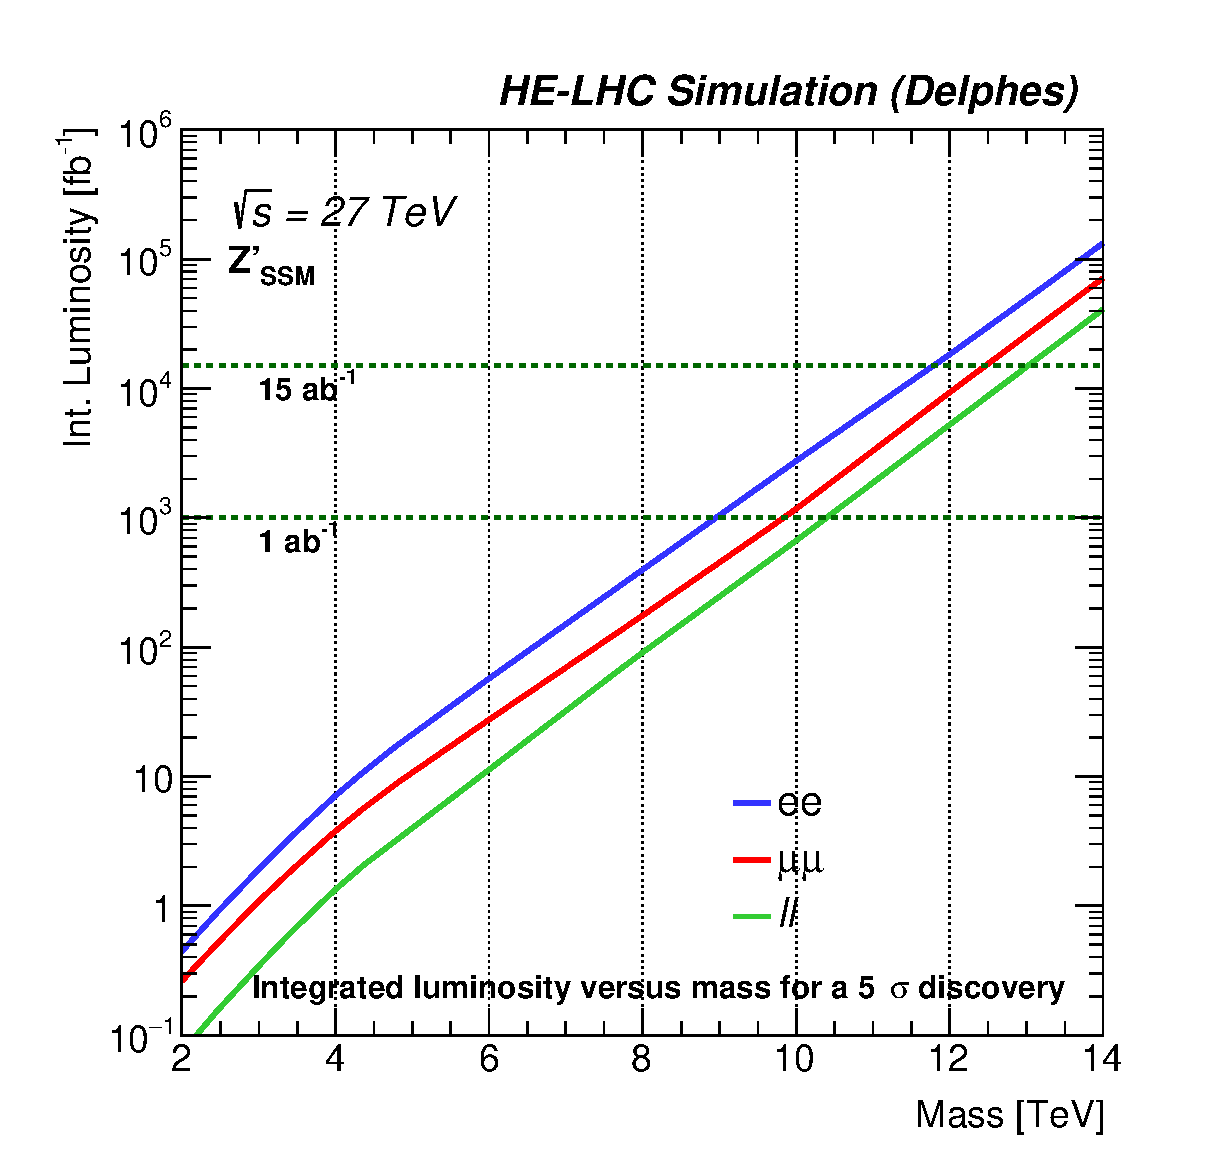
\includegraphics[width=0.45\columnwidth]{\main/section7OtherSignatures/img/DiscoveryPotential_ll_comb_rootStyle.eps}
  \caption{Exclusion limit versus mass for the dilepton (ee,$\mu\mu$) channel (left) and luminosity for a $5\sigma$ discovery (right) comparing ee,$\mu\mu$ and combined channels. }
  \label{fig:leptonicresonances:resultsll}
\end{figure}

\begin{figure}[htbp]
  \centering
    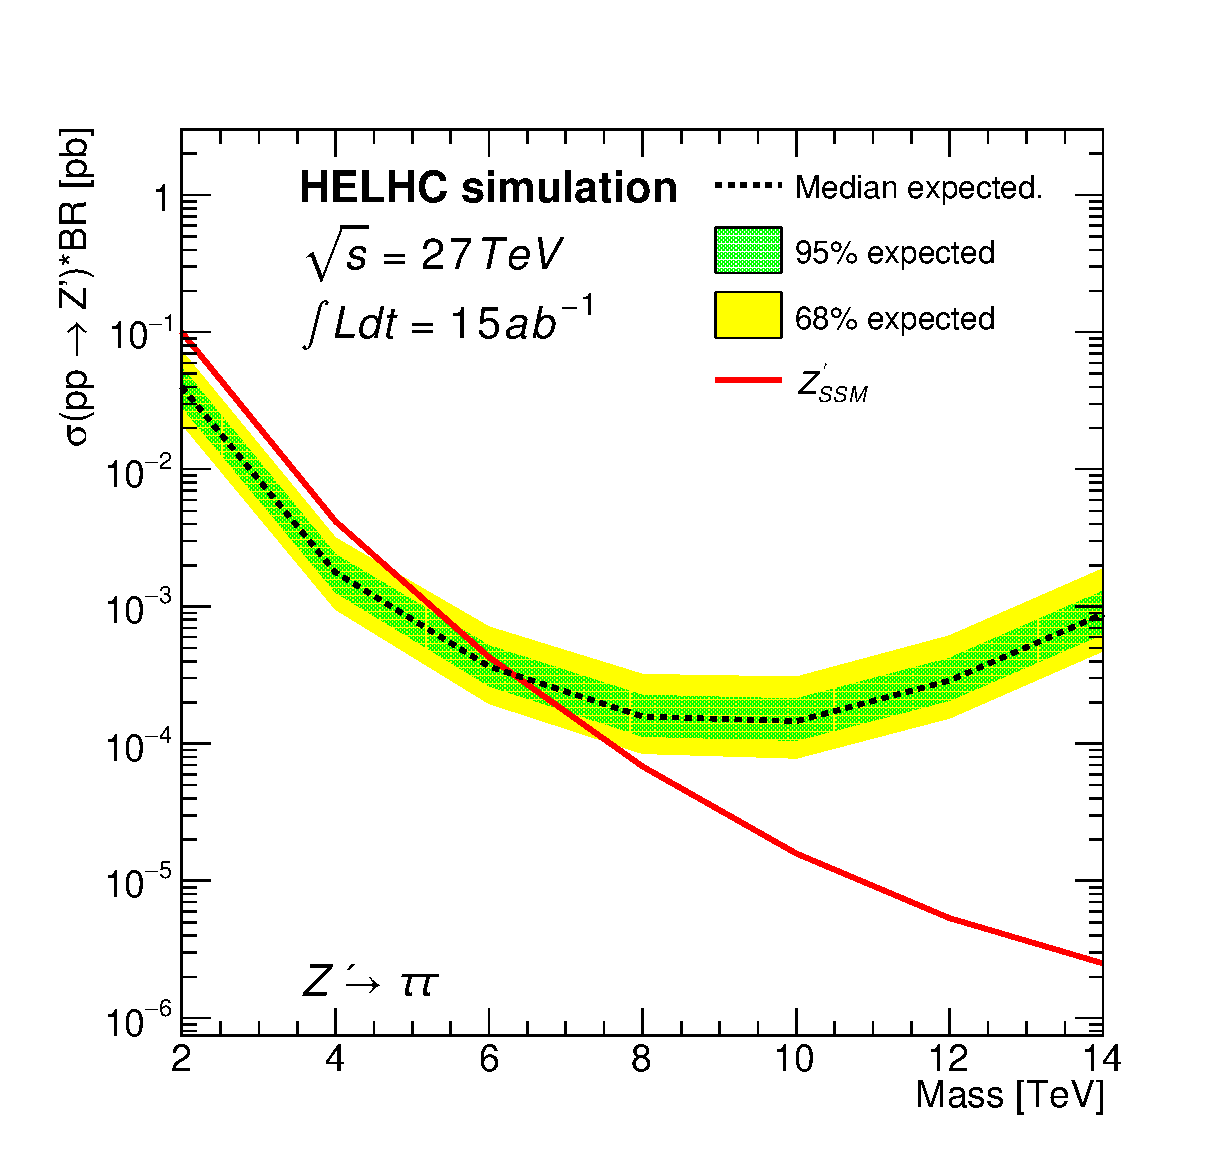
\includegraphics[width=0.45\columnwidth]{\main/section7OtherSignatures/img/lim_Zprime_tautau_helhc_v01.eps}
    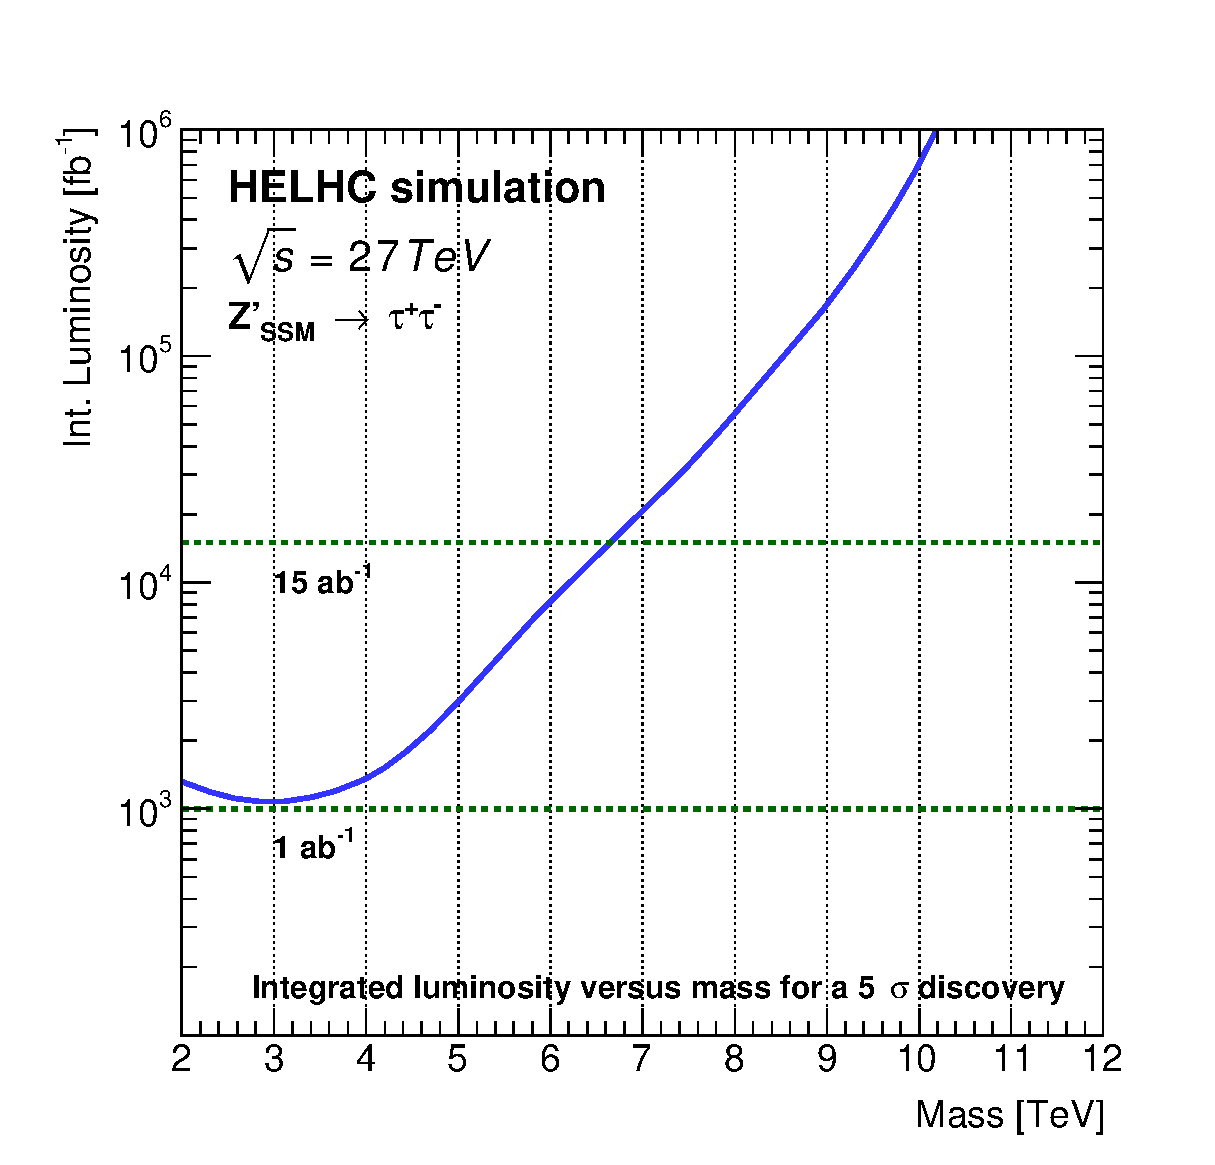
\includegraphics[width=0.45\columnwidth]{\main/section7OtherSignatures/img/DiscoveryPotential_tautau_rootStyle.eps}
  \caption{Exclusion  Limit versus mass for the ditau channel (left) and luminosity for a $5\sigma$ discovery (right). }
  \label{fig:leptonicresonances:resultstautau}
\end{figure}
